\section{Metrics and benchmarks}
Before put the hands on topic modelling, it is useful to define some metrics to test and benchmark the model.

Looking at the cluster side of the network, the outputs are sets of samples, the clusters. One can state the the model works if all, or at least the majority, of samples in the same cluster share some property. Here the tissue is considered as property.

Note that this work's model is a non supervised one, but a ground truth is available from metadata. So every sample has a certain probability to have a certain property (the true tissue label), let's call this $P(C)$ and a certain probability of being in a cluster (model's output), let's call this $P(K)$.

It is possible to define some quantities, the homogeneity
\begin{equation}\label{eq:homogeneity}
    h=1-\frac{H(C|K)}{H(C)}
\end{equation}
defining the entropy
\begin{equation}\label{eq:hck}
    H(C|K)=\sum_{c\in \mathrm{tissues},\\ k \in \mathrm{clusters}}\frac{n_{c k}}{N}Log\left(\frac{n_{c k}}{n_k}\right)
\end{equation}
where $n_{c k}$ is the number of nodes of type $c$ in cluster $k$, $N$ the number of nodes and $n_k$ the number of nodes in cluster $k$. It is evident that if all nodes inside cluster $k$ are of the same type $c$ $n_{c k}=n_{k}$, $H(C|K)=0$ and $h=1$, it is actually a complete homogeneous situation.

Another quantity can be defined and it is completeness:
\begin{equation}\label{eq:completness}
    c=1-\frac{H(K|C)}{H(K)},
\end{equation}
$H(K|C)$ is defined in the same way as~\ref{eq:hck}. Completeness measures if all nodes of the same type are in the same cluster.

Ideally one wants a method which output is both homogeneous and complete. So it is possible to define the V-measure, which is the harmonic average of the two:
\begin{equation}\label{eq:mutualinformation}
    MI=2\frac{h c}{h + c},
\end{equation}
which is actually the mutual information between $P(C)$ and $P(K)$~\cite{rosenberg2007v}.

In the next sections will be studied also the maximum fraction of label in the same cluster \(max_{c\in k}\frac{n_{c k}}{n_k}\).
Also the number of different labels in the same cluster will be studied.

\begin{figure}[htb!]
    \centering
    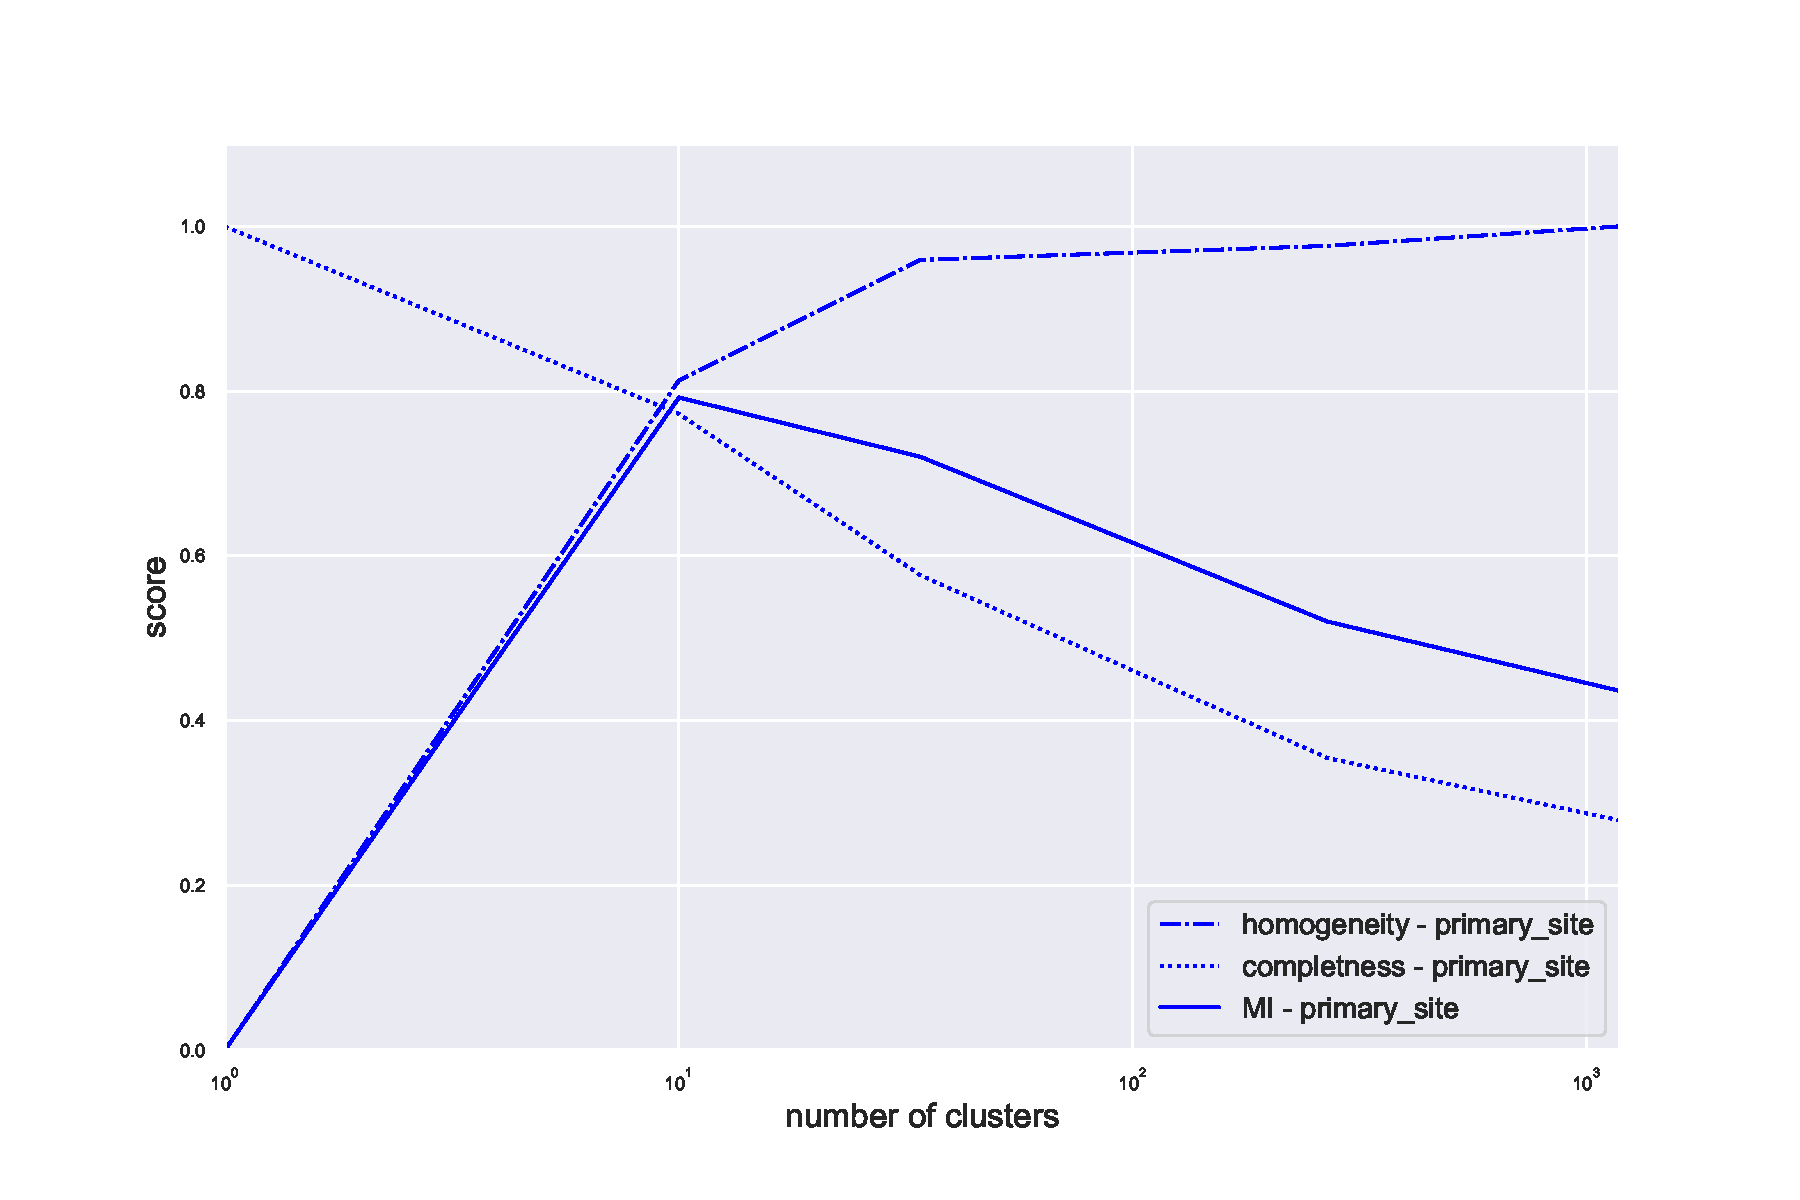
\includegraphics[width=0.9\linewidth]{pictures/topic/gtex/oversigma_10tissue/metric_scores_primarysite.pdf}
    \caption{Scores across hierarchy. The mutual information is the harmonic average between homogeneity and completeness}
    \label{fig:topic/metric_scores_primarysite}
\end{figure}